
\section{Energy Scale Calibrations} \label{CombinedEnergyModel}
%Discuss recombination physics and the ability to turn the now (emphasis on this, since it is how we transition from the previous section) corrected data into an combined energy scale.  Then basically cover recombination physics (prob in Attila's thesis) and Doke plot from my Doke plot write up.

The correction methods discussed in Chapter~\ref{StandardCalibrations} allow us to use two spatially independent gain factors to convert the S1 and S2 signals into the number of photons and the number of electrons produced by an event anywhere in the detector. In this chapter, we will present a combined energy model which uses the number of photons and electrons produced to determine the energy deposited during an event before discussing methods to measure the individual gain factors. 


\subsection{Combined Energy Model} \label{RecombSec} 


Energy from a particle interaction produces excited xenon atoms (Xe$^*$), ionized xenon atoms (Xe$^+$), and heat.  The heat released in the interaction is not observed in LUX.  For electron recoil events this lost energy is negligible, but for nuclear recoil it is not.

\begin{figure}[h]\centering
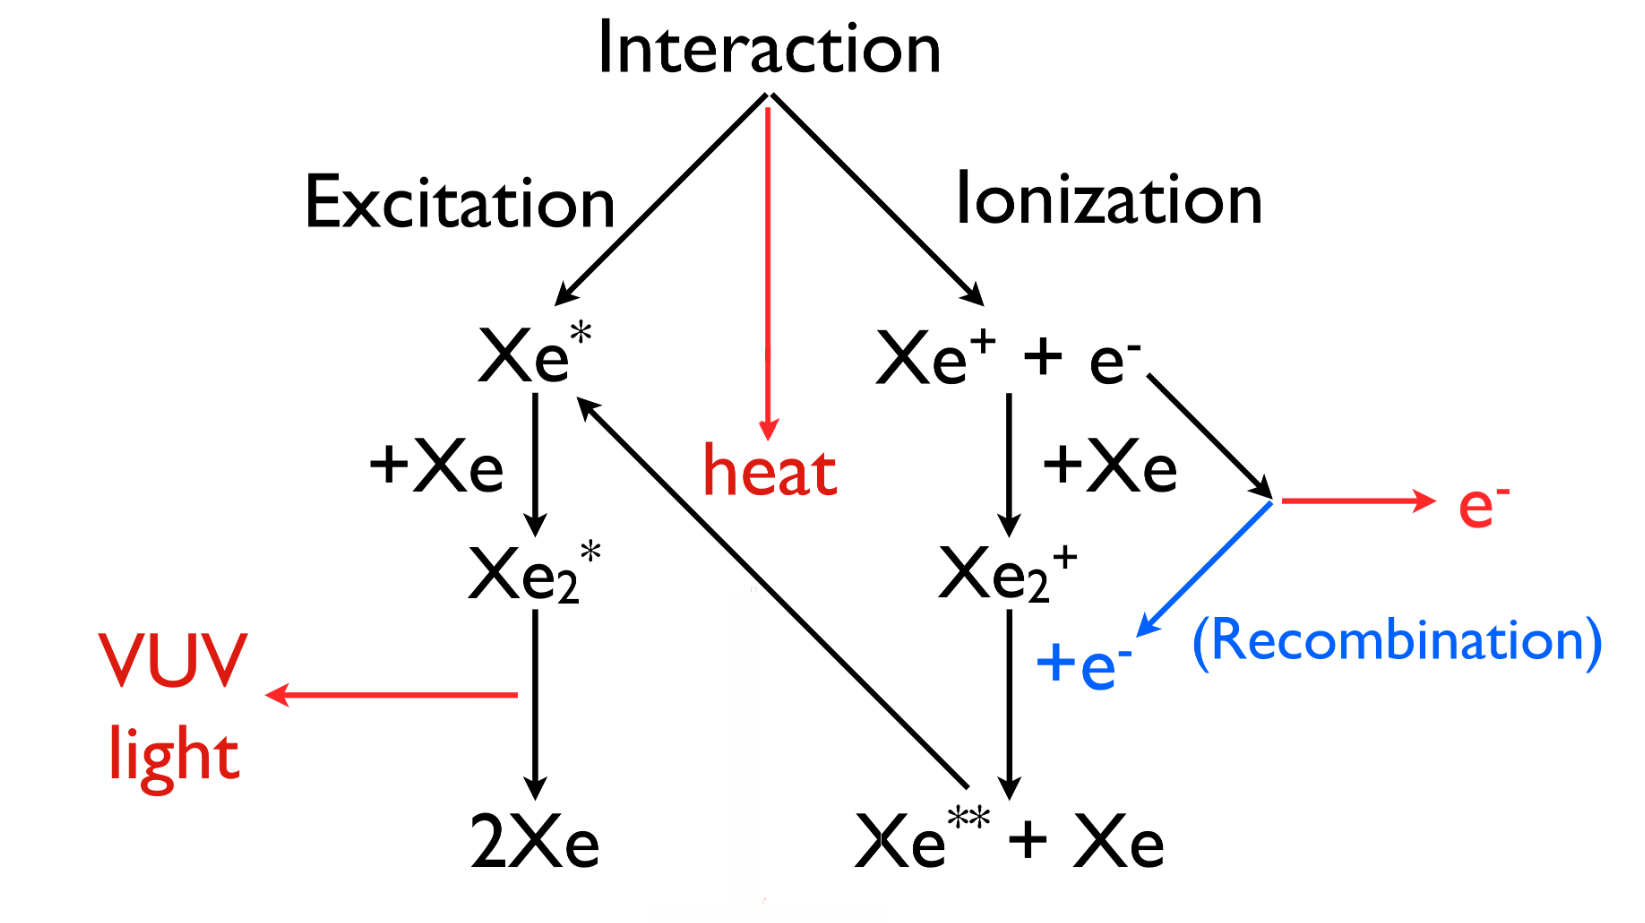
\includegraphics[scale=0.3]{InteractionPhysics.png}
\caption{Depiction of particle interaction and the production of xenon excitons, ionized xenon, electron, photons, and heat~\cite{Phelps}.}
\label{fig:InteractionPhysics}
\end{figure}

The excited xenon atoms combine with ground state xenon atoms to form xenon dimers (Xe$^*_2$).  These xenon dimers relax to two ground state xenon atoms, producing a 178 nm VUV photon.  This scintillation light is the first component of the S1 signal observed in the LUX detector. The ionization of xenon atoms releases free electrons.  These free electrons have a chance to recombine with the positively charged xenon ions, producing additional excitons which contribute to the S1 signal. Therefore, with the probability of an ion recombining represented as $R$, the number of photons produced in an interaction is given by the initial number of excitons produced plus the number of ions which recombine,
\begin{equation}
N_\gamma = N_{ex} + R N_i = N_{i}  (\alpha + R).
\end{equation}
where $N_\gamma$ is the number of photons, $N_{ex}$ is the number of excitons, $N_i$ is the number of ions, and $\alpha \equiv \frac{N_{ex}}{N_i}$ is the exciton to ion ratio. 


%S2 signal

Free electrons which do not recombine drift to the liquid surface where the accelerate through the extraction field and produce the S2 signal.  The number of electrons produced in an interaction is given by the fraction of ions which do not recombine,
\begin{equation}
N_e = N_i(1-R).
\end{equation}
Nuclear recoils are more densely ionizing than electron recoils, leading to more recombination, and therefore more S1 and less S2 signal.  This distinction enables the discrimination method discussed in Section~\ref{DiscrimSec}.  Note that in addition to the dependence on the type of recoil, the probability of recombination depends on the electric field and the energy of an interaction, a property which is significant for the work in Chapter~\ref{Run04Corrections}.

The total energy deposited by an interaction is given by
\begin{equation} \label{EnergyOne}
E = \mathcal{L}^{-1} W (N_{ex} + N_i)
\end{equation}
where where $E$ is energy in keV, $\mathcal{L}$ is the Lindhard factor which compensates for heat loss, and $W$ and is work function for the creation of excitons and ions in liquid xenon. The work function has been measured to be  W=13.7$\pm$ 0.2 eV/quanta~\cite{Dahl}. 

%Talk about linhard factor here
In terms of the atomic mass ($A$), the atomic number ($Z$), and energy of the nuclear recoil ($E_{nr}$), the Lindhard factor is given by 
\begin{equation}
\mathcal{L}=\frac{kg(\epsilon)}{1 + kg(\epsilon)}
\end{equation}
where
\begin{equation}
k=0.133 \times Z^{2/3} \times A^{1/2}
\end{equation}
\begin{equation}
g(\epsilon)=3\epsilon^{0.15} + 0.7\epsilon^{0.6} +\epsilon
\end{equation}
\begin{equation}
\epsilon = 11.5 \times E_{nr} \times Z^{-7/3}.
\end{equation}  For ER events, L equals one, and for NR events L ranges between 0.1 and 0.2.

Sometimes, experiments use the effective Lindhard factor $L_{eff}$ (also known as relative scintillation efficiency), defined as the ratio of zero-field light yields of ER and NR events
\begin{equation}
L_{eff} = \frac{N_{\gamma,NR} E_{ER}}{N_{\gamma,ER} E_{ER}}
\end{equation}
where the energy is typically chosen to be a 122 keV gamma.

From Equation~\ref{EnergyOne} we see that the same number of electron and photons can produce different energy reconstruction depending on the type of recoil interaction.  To avoid ambiguity, the energy of an event is typically referred to in units of kilo electron-volts electron recoil equivalent (keVee) or kilo electron-volts nuclear recoil equivalent.  All of the data presented in this thesis is a product of electron recoil calibration sources, so it should be assumed that we are using units of electron-volts electron recoil equivalent unless other wise stated.

To make use of our combined energy model, we need to convert the S1 and S2 observables from units of photons detected (phd) to the number of photons and electrons produced by the interaction.  We do so by defining two gain factors.  The gain factor for the S1 signal is referred to as g$_1$, and is given by the ratio of the average numbers of photons produced by an interaction to the observed S1 signal,
\begin{equation}
\langle n_\gamma \rangle = \frac{ \langle S1 \rangle }{g_1}.
\end{equation}
Note that the g$_1$ gain factor allows the S1 signal to be written in terms of the number of photons produced
\begin{equation}
S1=g_1 n_\gamma = g_1 (N_{ex} + R N_i) = g_1 * (\alpha + R) N_i
\end{equation}
The size of g$_1$ is dependent on the light collection efficiency in the detector, and can be thought of as the probability of a photon from an interaction striking a PMT and producing a photo electron. 

The gain factor for the S2 signal is referred to as g$_2$, and is given by the ratio of the average numbers of electrons produced by an interaction to the observed S2 signal.  
\begin{equation}
\langle n_e \rangle = \frac{ \langle S2 \rangle }{g_2}
\end{equation}
As with the S1 signal, g$_2$ allows us to write the S2 signal in terms of the number of electrons produced by an interaction,
\begin{equation}
S2=g2 n_e=g_2 (1-R) N_i
\end{equation}
The size of g$_2$ is dependent on the efficiency at which electrons are extracted from the liquid xenon at the surface (the extraction efficiency), and the number of photo electrons detected per extracted electron (the single electron size).  

\subsection{Doke Plot Analysis of g$_1$ and g$_2$}

The gain factors g$_1$ and g$_2$ can be calculated by requiring that the combined energy model reproduce the true energy of two or more electron recoil sources that produce different light and charge yields.  In electron recoil events, the light yield and charge yield is a dependent on both the energy of an event, and the strength of the electric field in which the event occurred.  Therefore the same electron recoil source taken at two different drift field settings can be used to determine the value of $g_1$ and $g_2$ alone. Table~\ref{sources} lists the eight sources which were selected to measure $g_1$ and $g_2$ in LUX's Run03 campaign.  


\begin{center}
\begin{tabular}{ | c| c | c | c | }
\hline
Source & Energy [keV] & Decay Type & Data \\ \hline
$^{127}$Xe & 5.3 & L shell x-ray & Run03 Data \\ \hline
$^{83m}$Kr & 41.55 & IC & Run03 Calibrations \\  \hline
$^{131}$Xe & 163.9 & IC & Early Run03 Data \\  \hline
$^{127}$Xe & 208.3 (203 $\gamma$ and 5.3 x-ray) & $\gamma$-emission & Run03 Data \\  \hline
$^{129}$Xe & 236.1 & IC & Early Run03 Data  \\  \hline
$^{127}$Xe & 409 (375 $\gamma$ + 33.8 x-ray) & $\gamma$-emission & Run03 Data \\  \hline
$^{214}$Bi & 609 & $\gamma$-emission & Detector Background \\  \hline
$^{137}$Cs & 661.6 & $\gamma$-emission & Run03 Calibrations \\
\hline
\end{tabular}
\captionof{table}{Table of sources used in the Doke plot analysis..}
\label{sources}
\end{center}

We use a Doke plot technique to ensure the combined energy model reproduces the true energy of all eight sources~\cite{Doke,Dobi}.  Solving Equation~\ref{EnergyOne} for $\frac{S1}{E}$, we find
\begin{equation}\label{four}
\frac{S1}{E} = \frac{g_1}{W} - \frac{S2}{E}\frac{g_1}{g_2}
\end{equation}
which is the equation of a line with
\begin{subequations}
\begin{align}
y=\frac{S1}{E} \; , \; x=\frac{S2}{E} \\
b=\frac{g_1}{W} \\
m=\frac{g_1}{g_2}=\frac{b \times W}{g_2}
\end{align}
\end{subequations}
This motivates the creation of a "Doke Plot" in which we plot the mean light yield, $\frac{S1}{E}$, versus the mean charge yield, $\frac{S2}{E}$, for each line source to find the best fit for
\begin{subequations}\label{six}
\begin{align}
g_1 = b \times W \\
g_2 = \frac{b \times W}{m}
\end{align}
\end{subequations}

Diagonal cuts chosen by eye were used for initial event selection of the sources in Table~\ref{sources}. Next, we fit a rotated two dimensional Gaussian distribution to the corrected S1 and S2 spectra of each source to determine the mean and sigma of the S1 and S2 populations. Once the standard deviation of each population is determined, we refit the data using only events within $\pm$2$\sigma$ of the S1 and S2 Gaussians means to eliminate tails caused by backgrounds.  A linear fit of $\frac{\langle S1 \rangle}{E} = m \frac{\langle S2 \rangle}{E} + b$ is performed using the refit Gaussian means.  Once an initial best fit for $g_1$ and $g_2$ is found, we can produce a combined energy scale using Equation~\ref{EnergyOne}.  This combined energy spectrum has significantly better resolution than the individual S1 and S2 spectra, and allows us to improve our initial event selection by placing a $\pm$2$\sigma$ cut around the energy peaks.  We then refit S1 and S2 spectra once more with the improved event selection, and find new values for the best fit of $g_1$ and $g_2$.  This process of producing an energy spectrum to improve event selection is iterated five times, but quickly converges after the second iteration.

\begin{figure}[H]
\centering
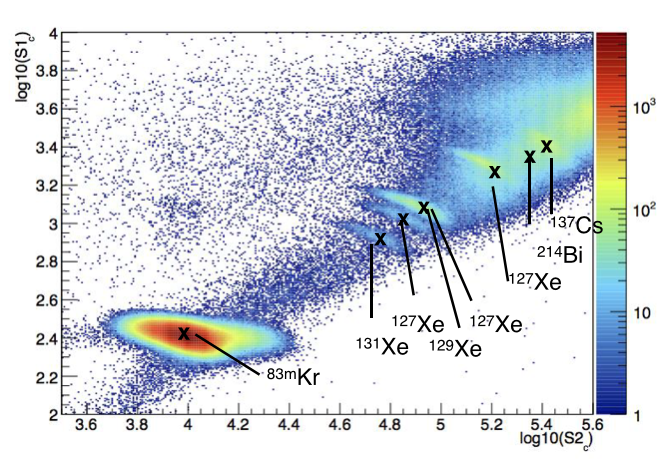
\includegraphics[scale=1]{Monoenergetic_gamma_sources.png}
\caption{S1 versus S2 density plot for all data that was used in Run03 Doke plot analysis.}
\label{alleventselection}
\end{figure}


\subsubsection{Doke Plot Systematic Errors}

There are a number of systematic errors on the S1 and S2 signals that must be considered when constructing the Doke plot.  One such error comes from the variation in single electron size over time, shown in Figure~\ref{SESizes}. The Doke plot uses data from many sources taken at different points in time, and therefore each point on the plot has a different single electron size.  Since we seek one value of g$_2$ which describes the all of the data, and since g$_2$ is equal to the extraction efficiency times the single electron size, the variation in single electron size must be included in the S2 error bars.

\begin{figure}[H]
\centering
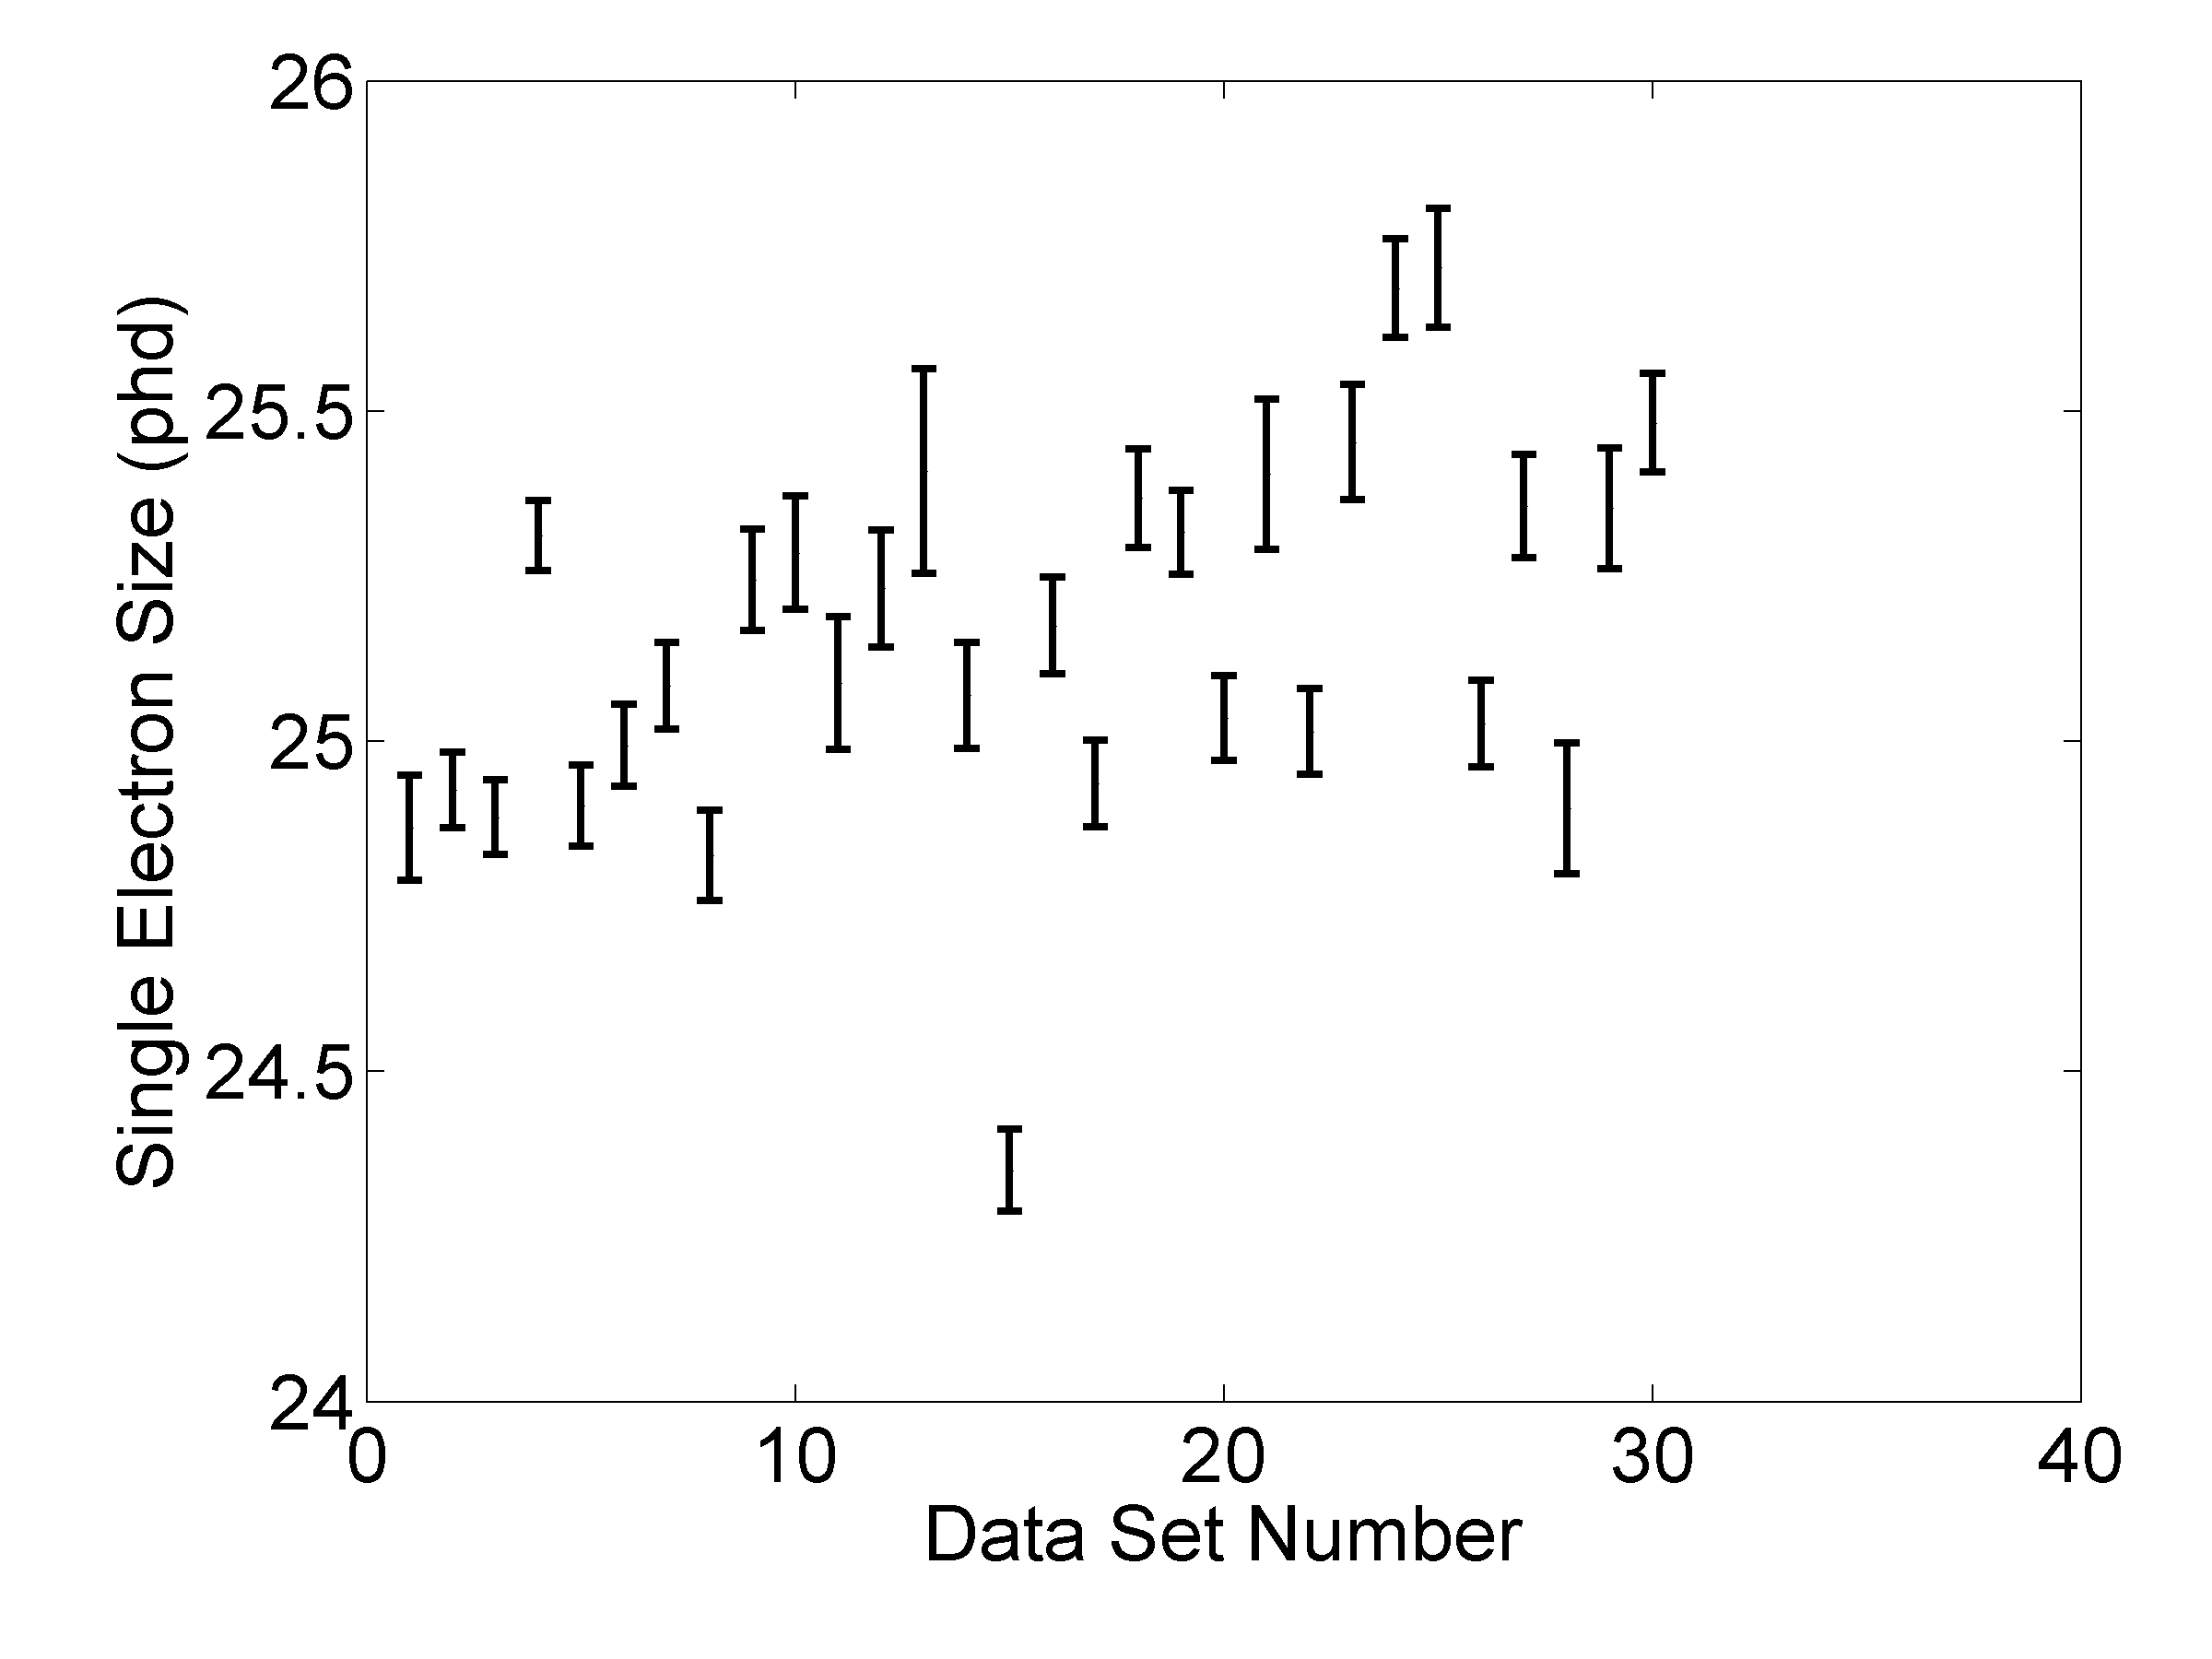
\includegraphics[scale=0.4]{SESizes.png}
\caption{Single electron sizes for all $^{83m}$Kr data sets over the course of LUX's Run03 data taking campaign.}
\label{SESizes}
\end{figure}


Another source of error is introduced by variations in the position dependent pulse area corrections.  Systematic variations in the correction maps lead to variation in the corrected S1 and S2 signals over time.  This adds a systematic error to all of our data points in the Doke plot which can be measured using the standard deviation of the corrected $^{83m}$Kr S1 and S2 peaks over time.  We assume that the size of this systematic error scales linearly with S1 and S2 size for the non-$^{83m}$Kr data points. 

\begin{figure}[H]
\centering
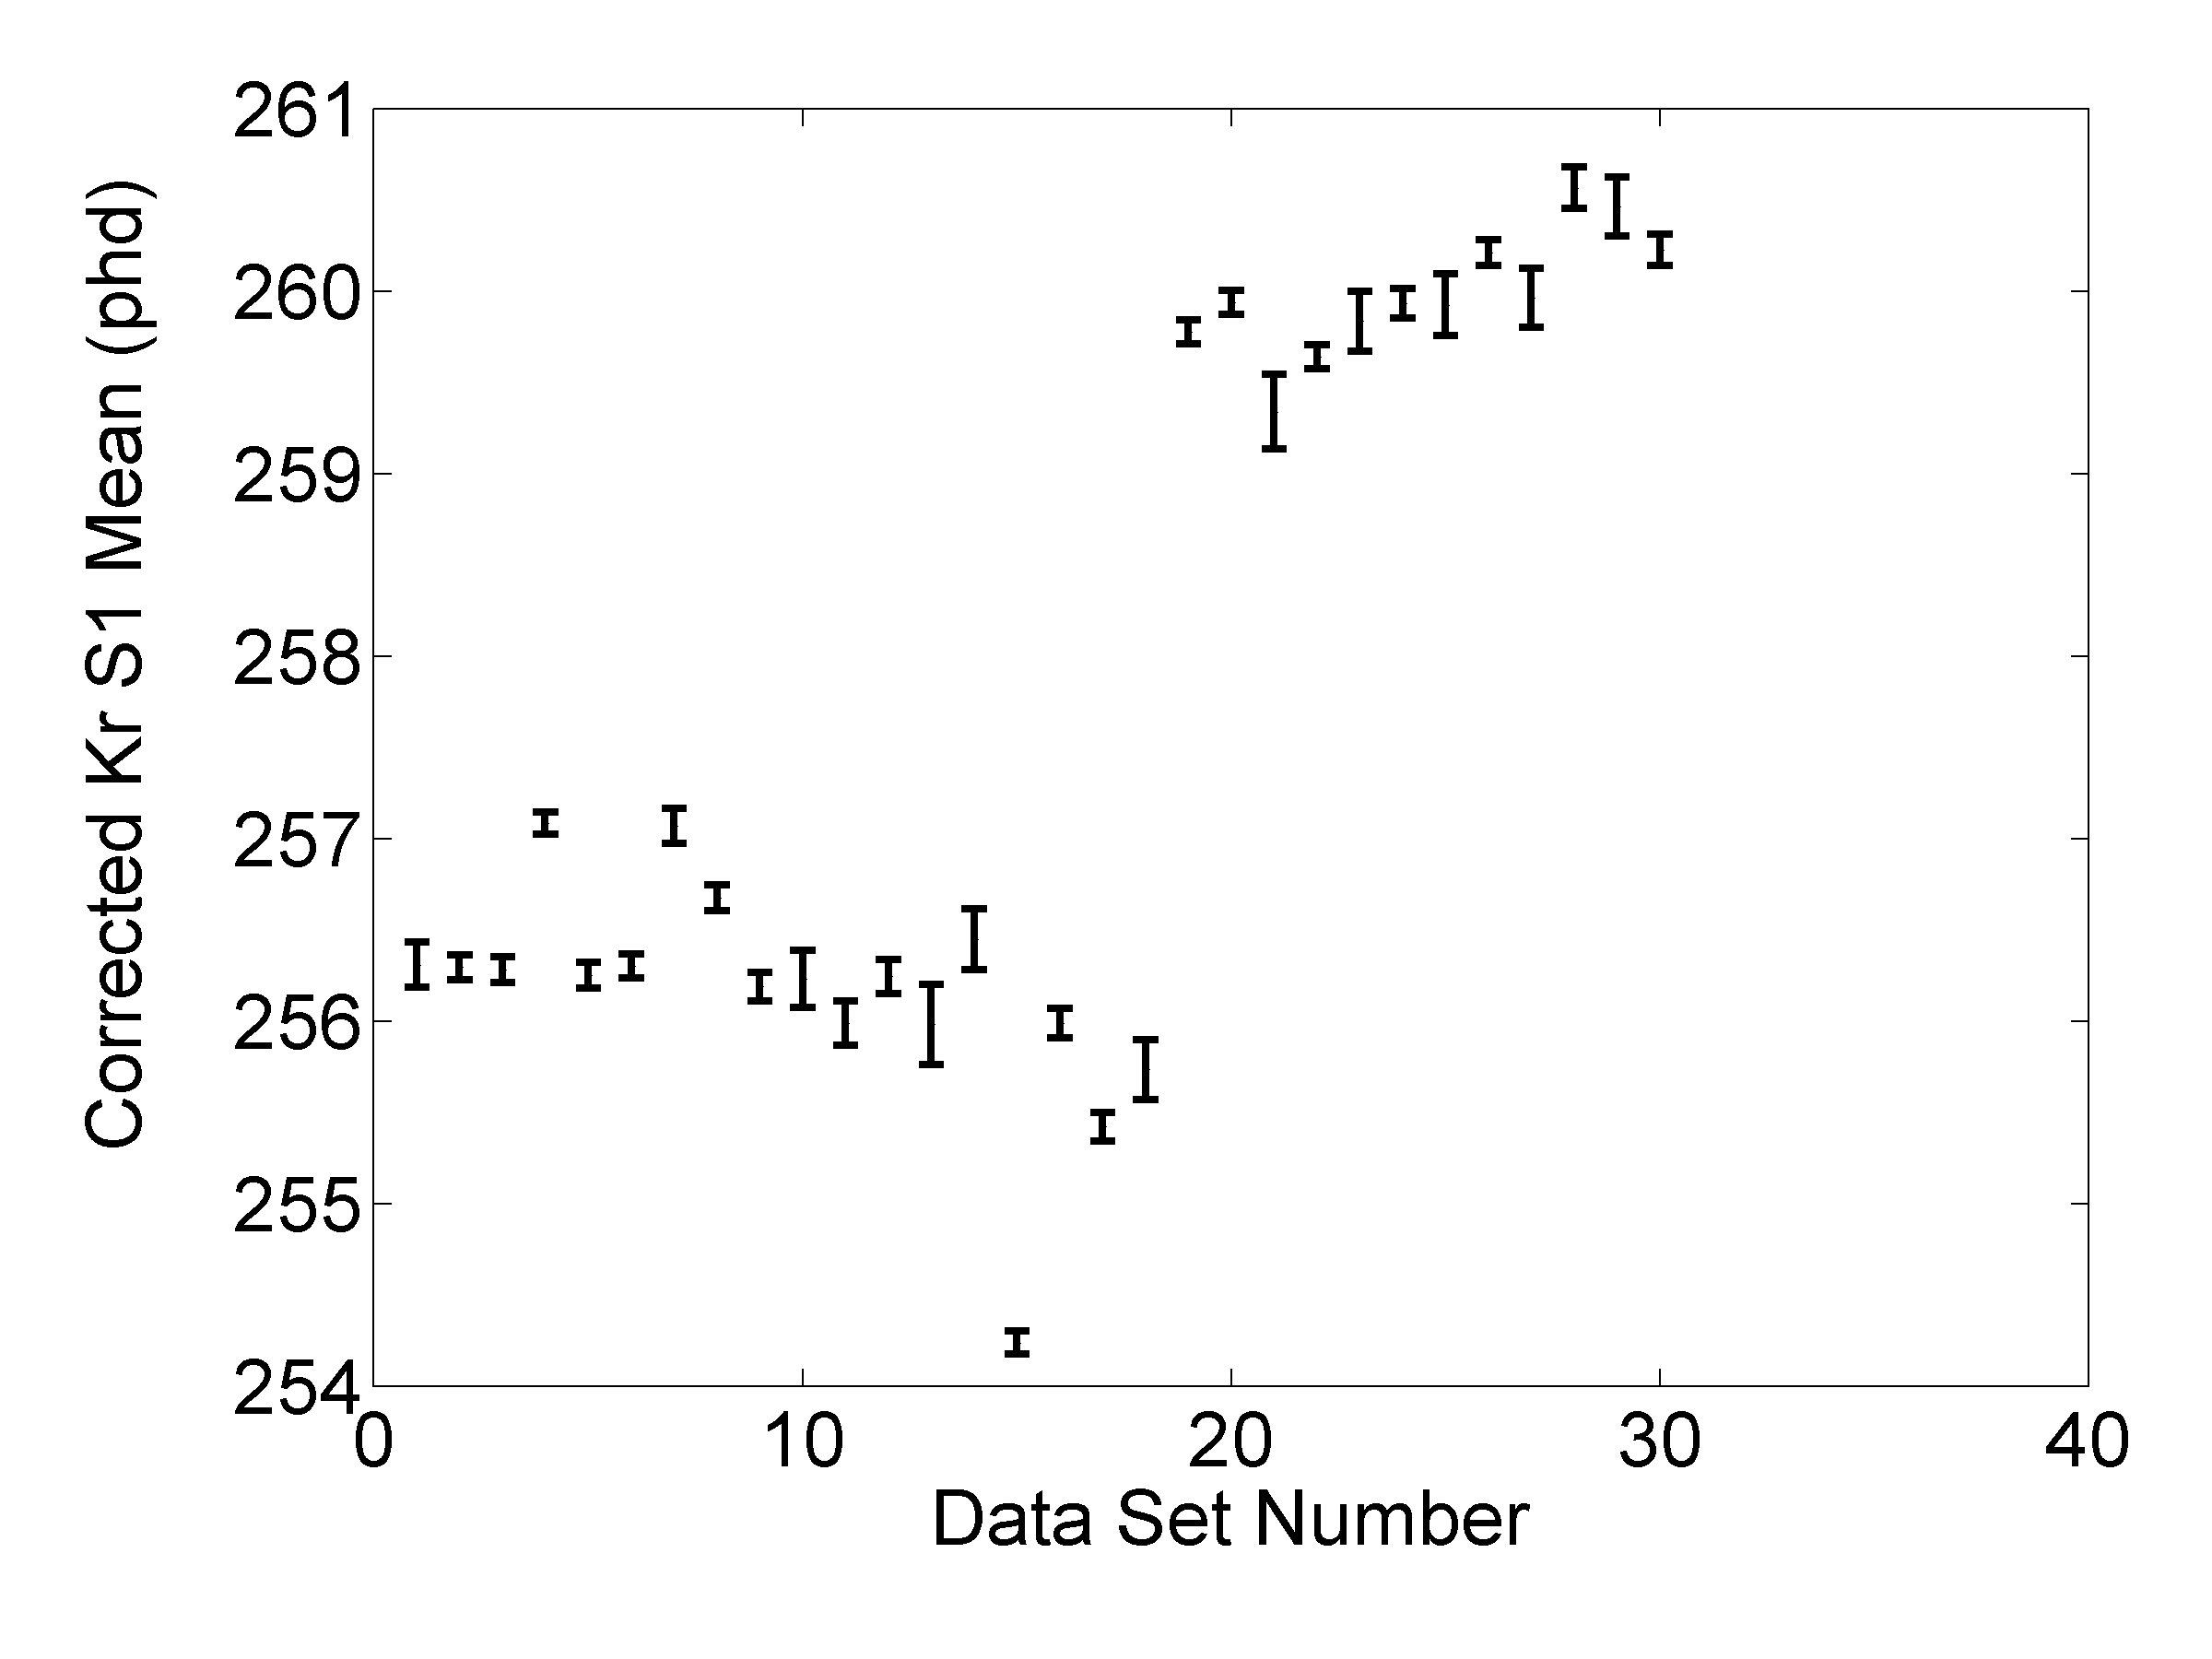
\includegraphics[scale=0.4]{S1Variation.png}
\caption{Corrected S1 peaks for all $^{83m}$Kr data sets at 170 V/cm field strength.  The step near data set 20 is due to an update of the S1 XYZ corrections map.  This effect is accounted for in our systematic errors}
\label{S1Variation}
\end{figure}


\begin{figure}[H]
\centering
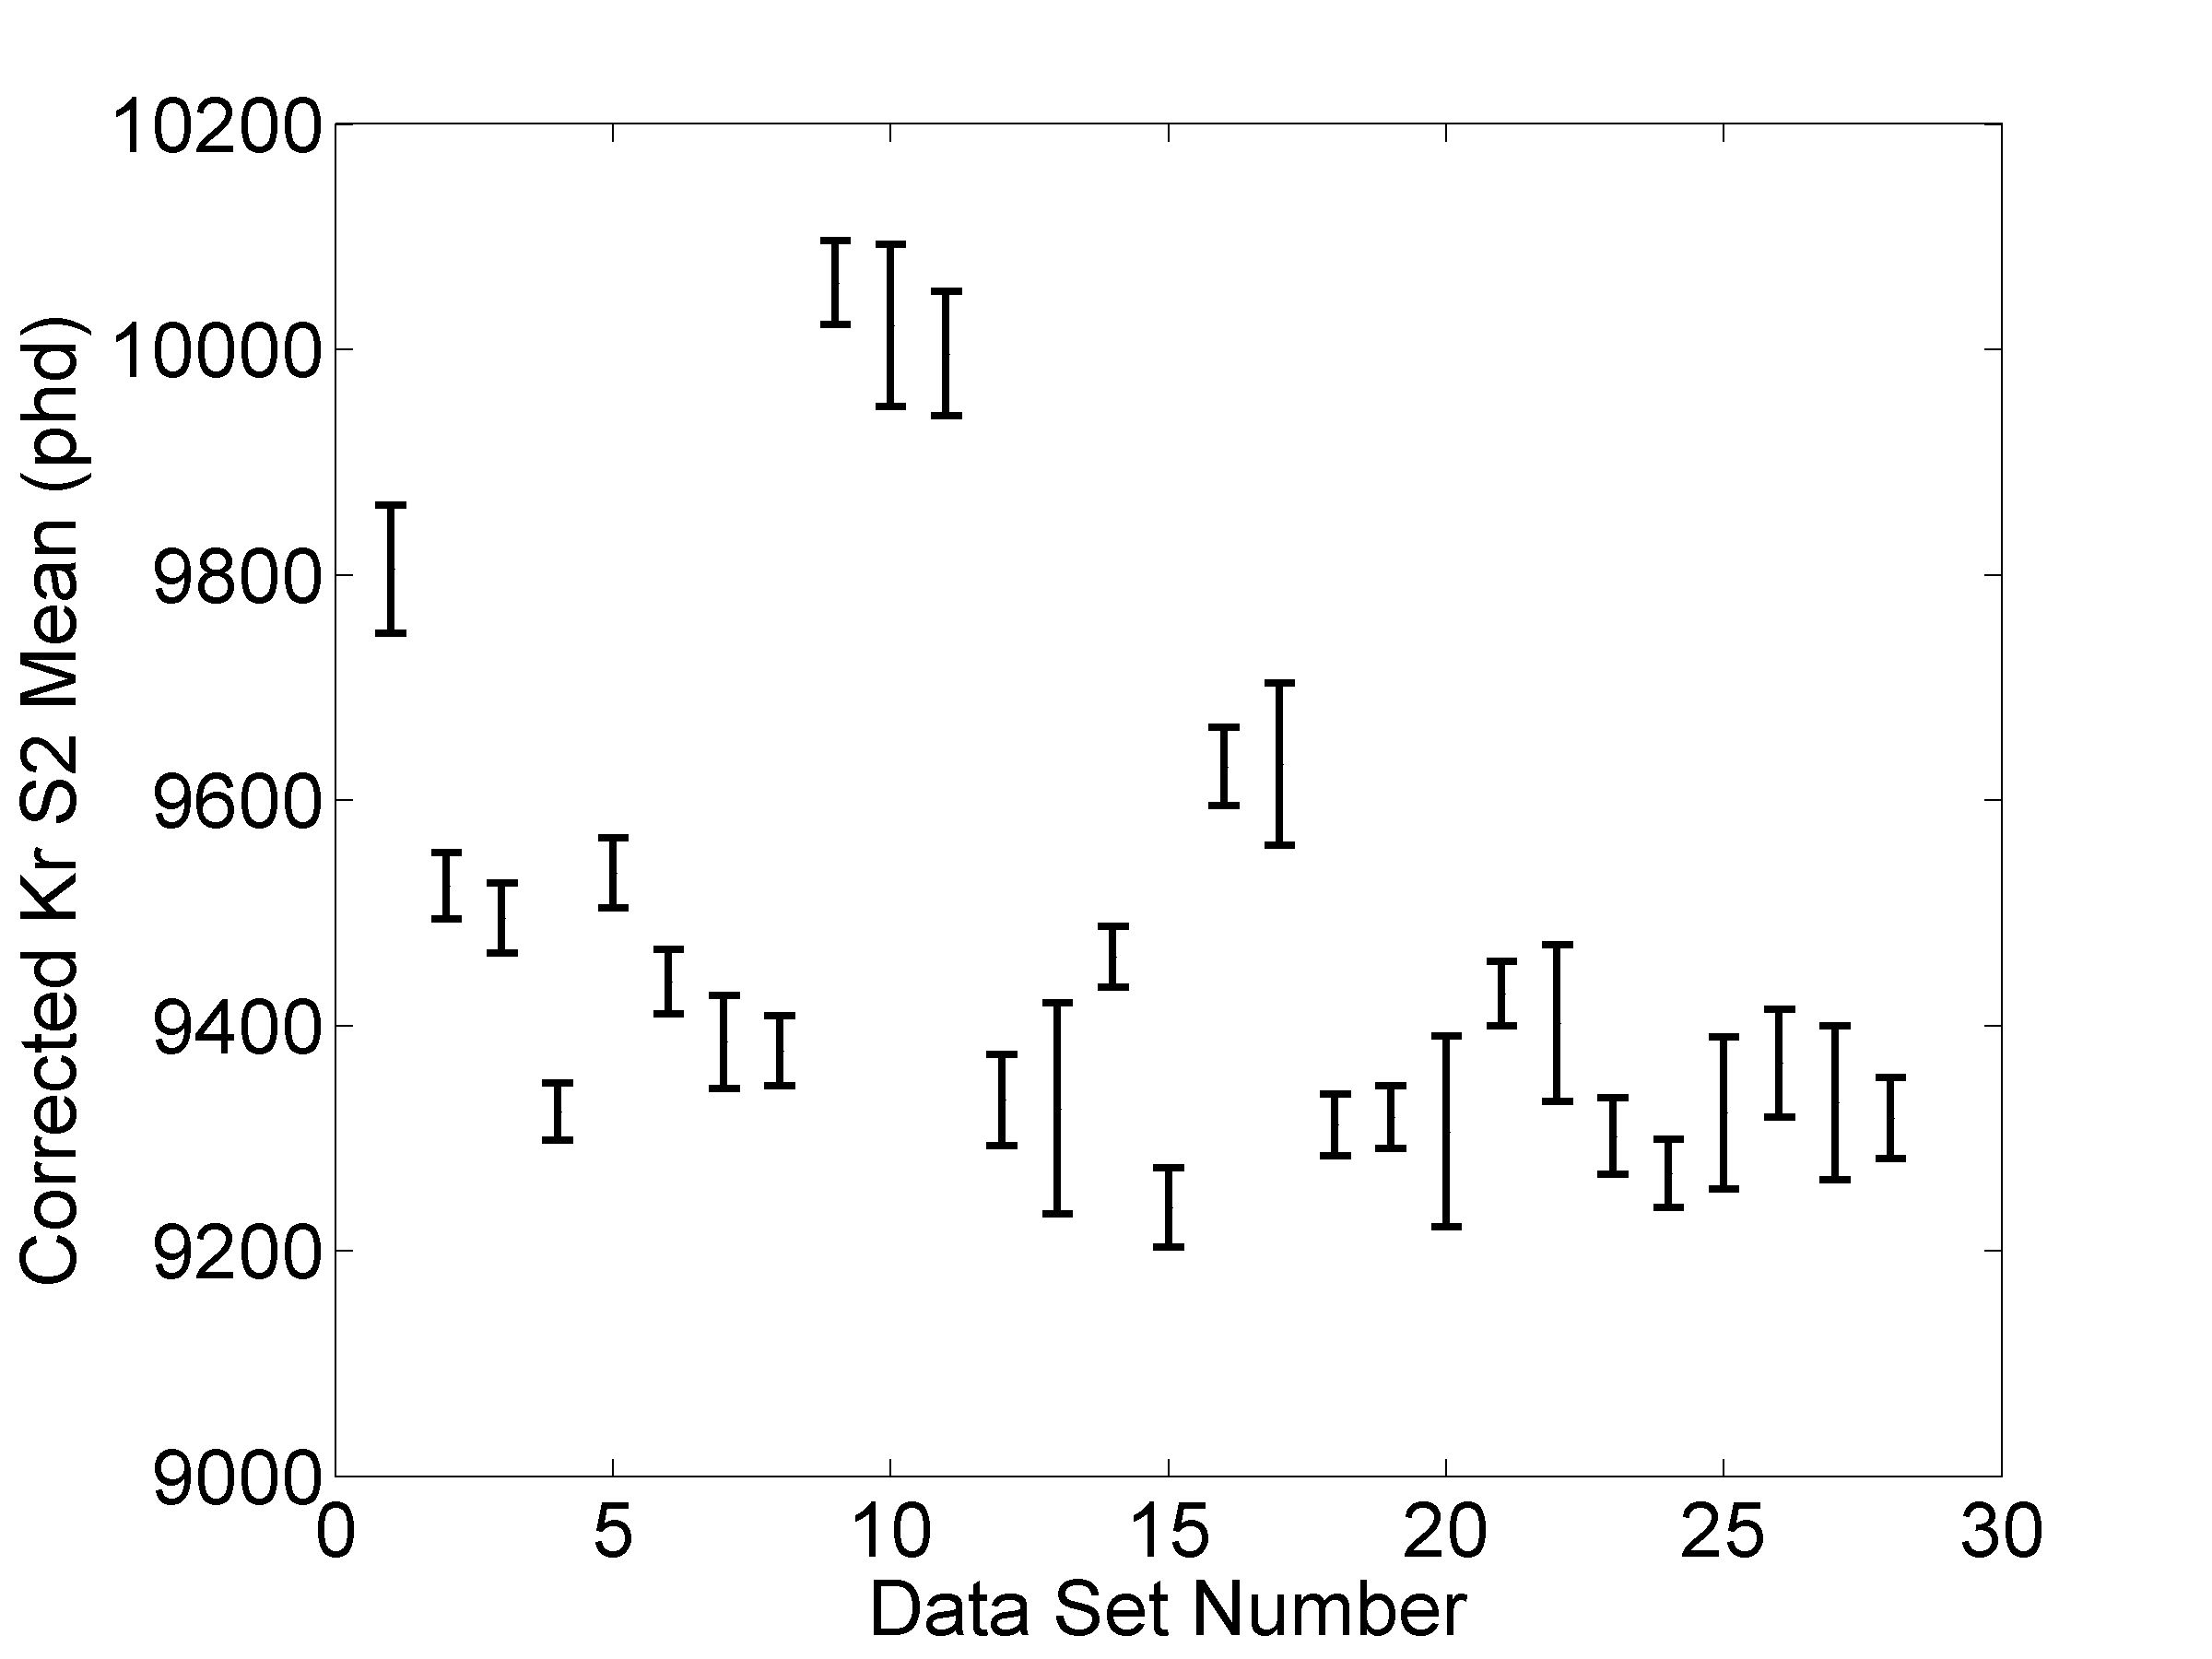
\includegraphics[scale=0.4]{S2Variation.png}
\caption{Corrected S2 peaks for all $^{83m}$Kr data sets at 170 V/cm field strength.}
\label{S2Variation}
\end{figure}

Additionally, there is a small difference in the measurement of $n_e=\frac{S2}{SE}$ for each Doke plot point when using both PMT arrays or using the bottom PMT array only. The number of electrons produced by a particle interaction is independent of how many PMTs observe the interaction, so this discrepancy can only be due to systematic errors which are likely produced by the PMT arrays saturating at high energies.  The size of this discrepancy is also included in the systematic error  of each point. 

\subsubsection{Doke Plot Results}


The Doke plot produced by the analysis described in the preceding sections is shown
in Figure~\ref{DokePlot}.  The best fit parameters for the Doke plot are high correlated.  To account for this the errors on the fit are calculated using a Markov chain Monte Carlo.  The covariance matrix produced after five thousand trials is used as for error measurement on each parameter.  We get a best fit of $g_1= 0.117 \pm 0.003$ and $g_2=12.1 \pm 0.8$.  This value of $g_2$ corresponds to an extraction efficiency of $EE = 0.491 \pm 0.032$.

In Figure~\ref{Run03EnergySpectrum} we use the best fit parameters from the Doke plot to produce energy spectra for each line source used in this analysis.  Sources that are below the line on the Doke plot have energy peaks that are lower than expected, and sources that are higher than the line on the Doke plot have energy peaks that are higher than expected.

%Show final Doke plot here
\begin{figure}[H]
\centering
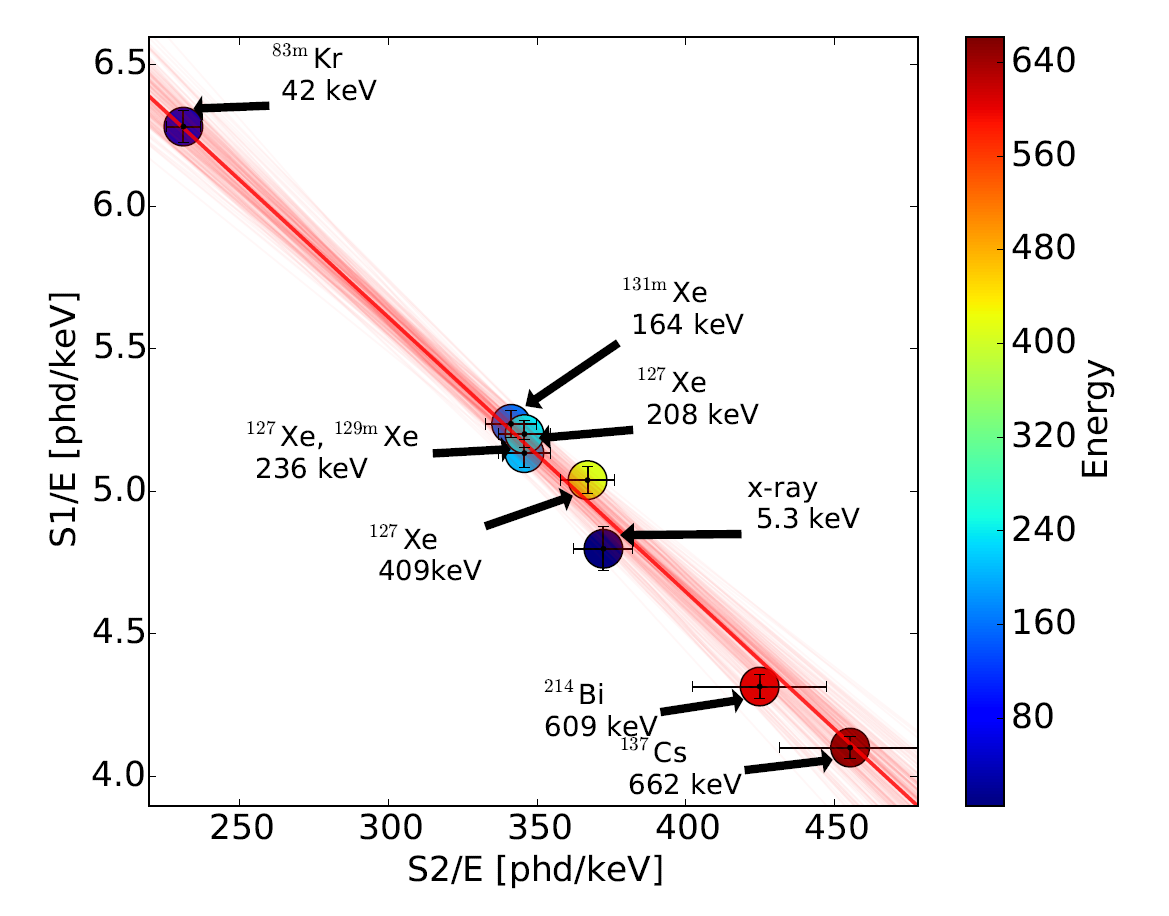
\includegraphics[scale=0.3]{DokePlot.png}
\caption{The Doke plot from this analysis.  The red faded red lines indicate the result of each MCMC trial, while the dark red line indicates the best fit result.  The energy of each source is indicated by the point's color.}
\label{DokePlot}
\end{figure}

%Show correlation plot here
\begin{figure}[H]
\centering
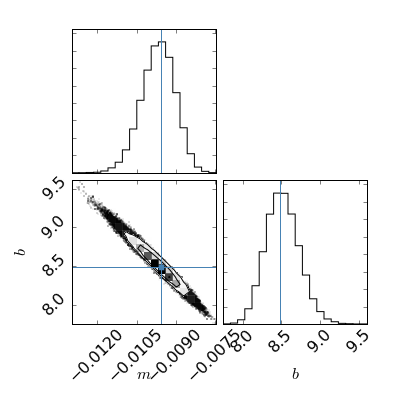
\includegraphics[scale=0.5]{DokeTrianglePlot.png}
\caption{A triangle plot showing the correlation between the fit parameters during the MCMC process. A projection of the fit results onto each axis is shown above and next to the triangle plot.}
\label{Corr}
\end{figure}


%Show energy spectrum here
\begin{figure}[H]
\centering
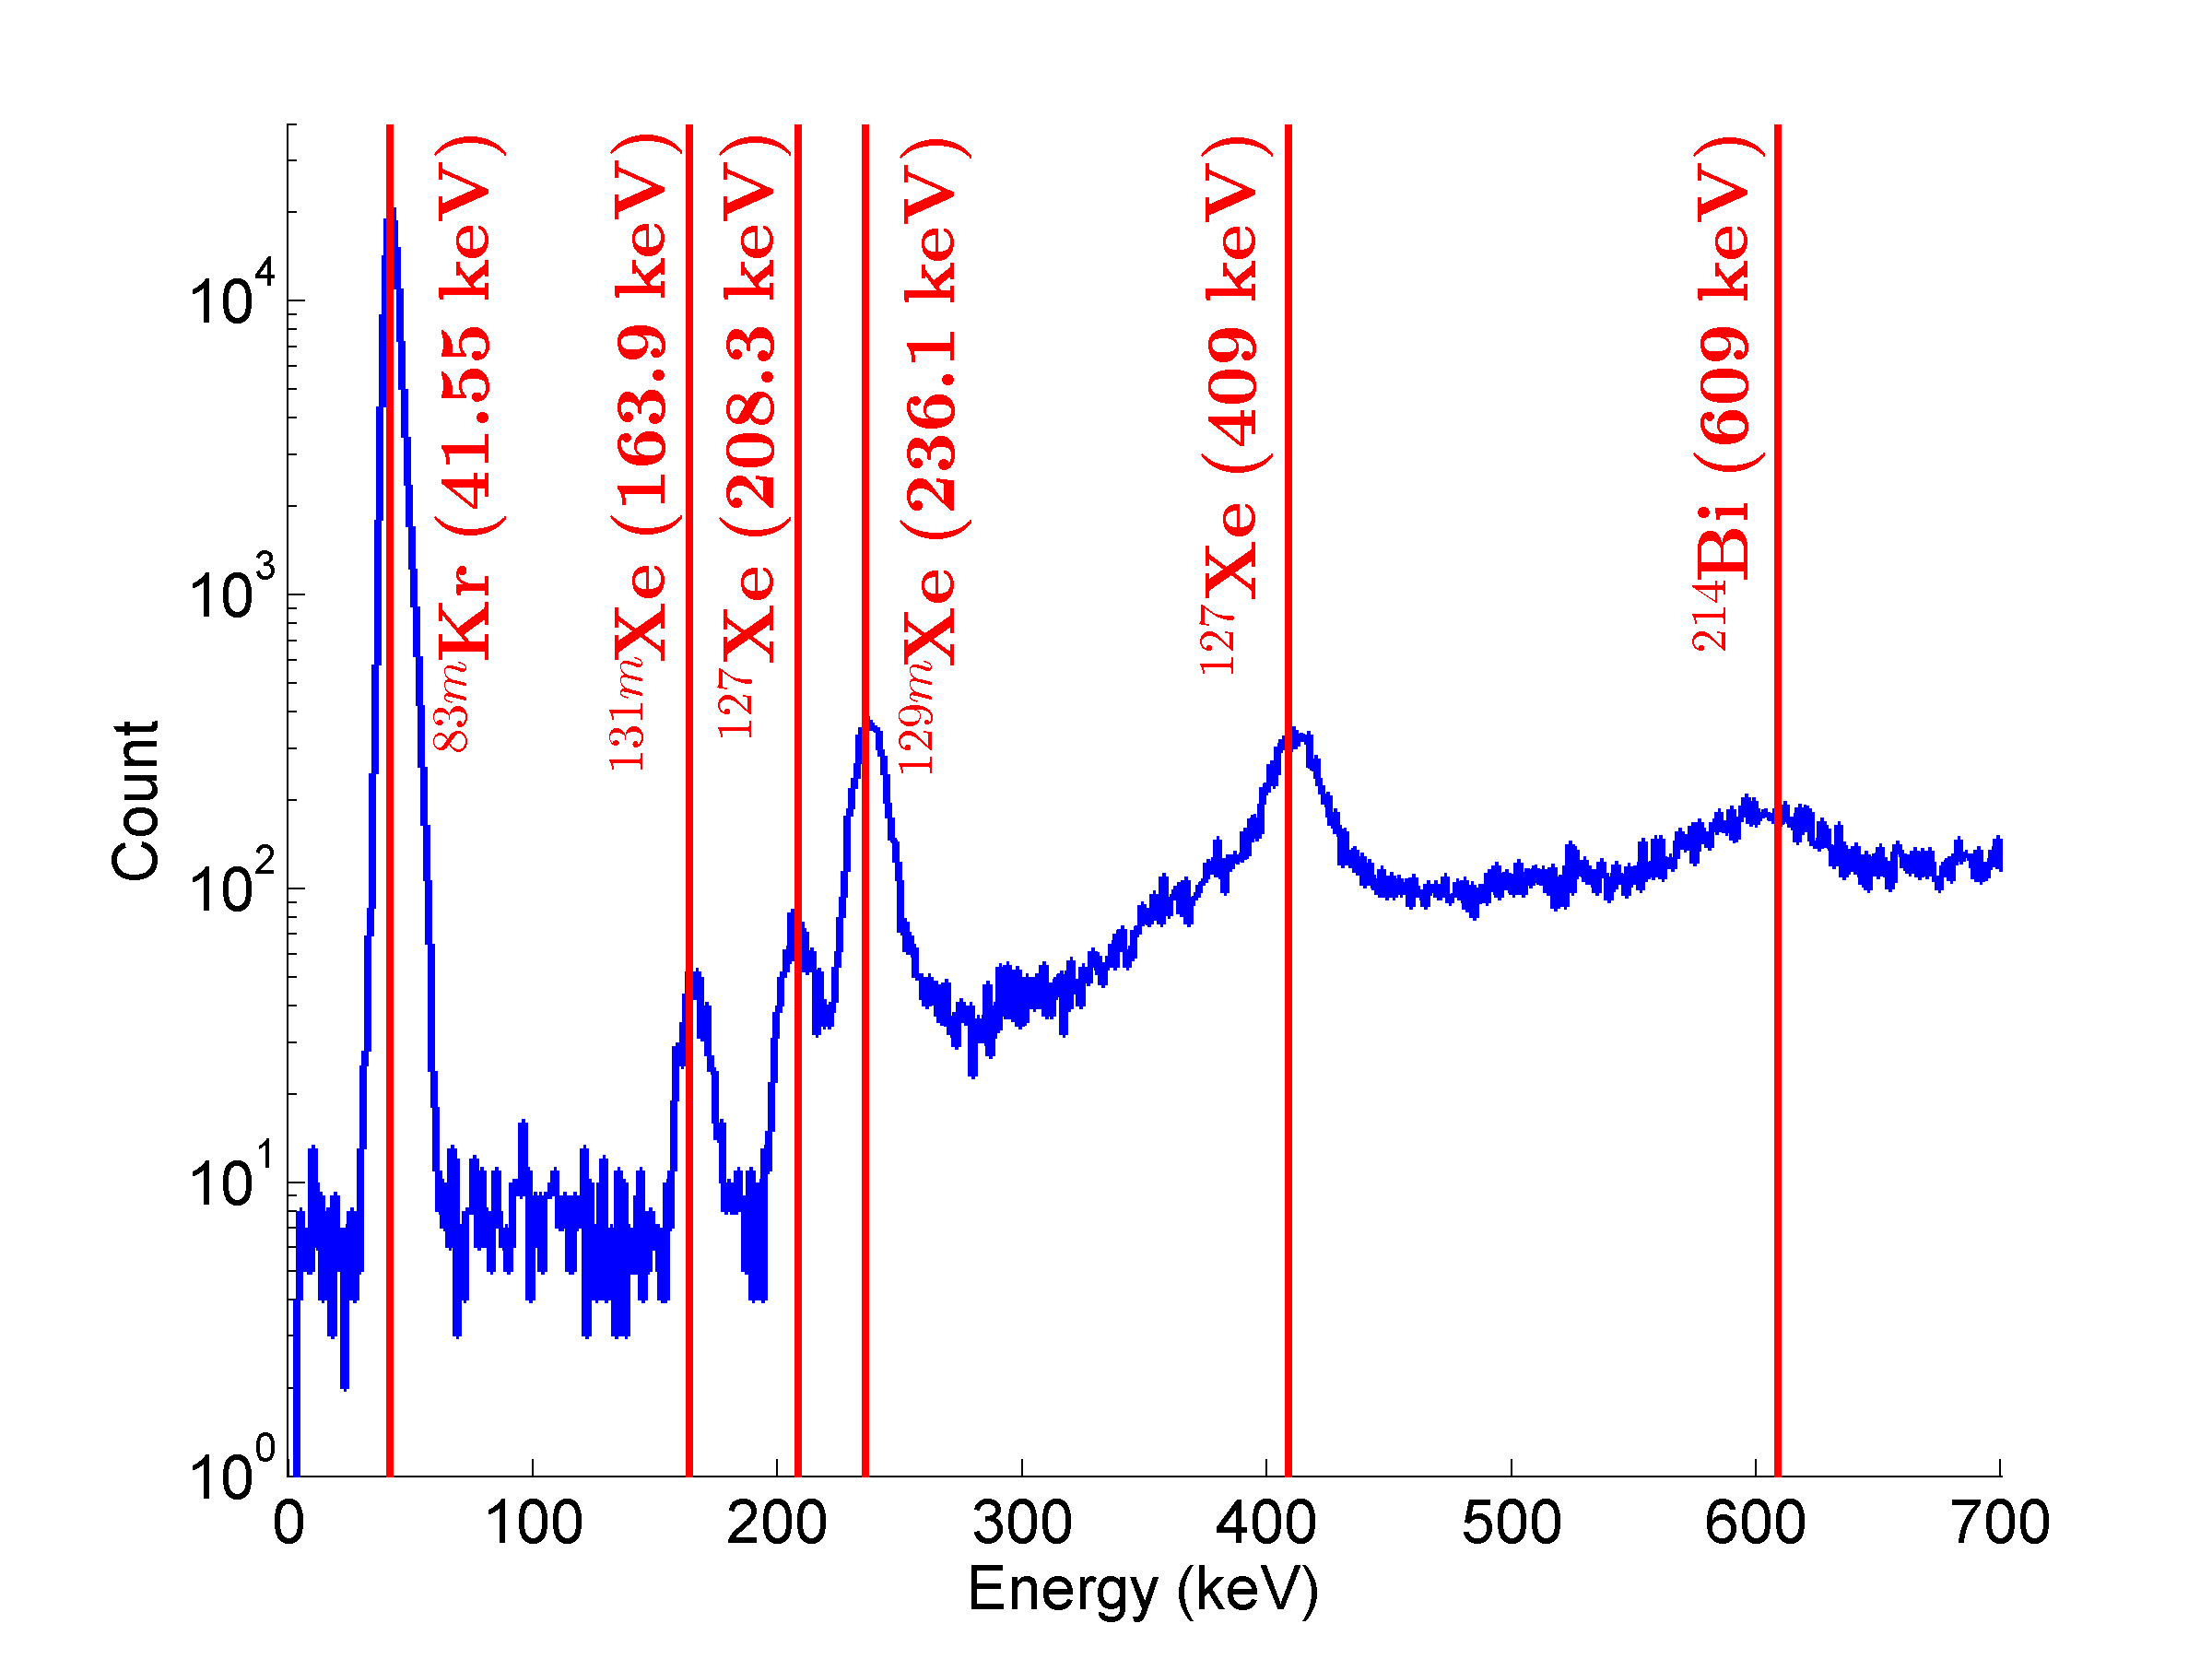
\includegraphics[scale=0.4]{WS_Spectrum.png}
\caption{The energy spectrum of LUX's Run03 data after using the g$_1$ and g$_2$ values from the Doke plot analysis}
\label{Run03EnergySpectrum}
\end{figure}


\newpage 

\subsubsection{Recombination Fluctuations from Doke Plot Data}

Using the methods from cite{Dobi} and the data from this Doke plot analysis we can determine recombination fluctuations ($\sigma_{R}$) as well as fluctuations in counting photons ($\sigma_{n_{\gamma Det}}$) and electrons ($\sigma_{n_{e Det}}$) due to detector resolution.  The relevant equations are

\[\sigma_{R}^2 = \frac{1}{2}( \sigma_{n_{\gamma Det}}^2 + \sigma_{n_{e Det}}^2 - \frac{\sigma_{E}^2}{W^2}) = \frac{1}{2}(\frac{\sigma_{S1}^2}{g_{1}^2} + \frac{\sigma_{S2}^2}{g_{2}^2} - \frac{\sigma_{E}^2}{W^2}) \]
\[ \sigma_{n_{\gamma Det}}^2 = \frac{\sigma_{S1}^2}{g_{1}^2} - \sigma_{R}^2 \]
\[ \sigma_{n_{e Det}}^2 = \frac{\sigma_{S2}^2}{g_{2}^2} - \sigma_{R}^2 \]


where $\frac{\sigma_{S1}^2}{g_{1}^2}$, $\frac{\sigma_{S2}^2}{g_{2}^2}$, and $\frac{\sigma_{E}^2}{W^2}$ can be measured with Gaussian fits to the S1, S2, and energy spectra for each point on the Doke plot.  The results of this analysis are shown in Table~\ref{SigR}.  The results included here are the outcome after setting the fitting window by eye in a way which eliminates the most background events while maintaining the majority of each spectrum's peak.  

\begin{center}
\begin{table}[H]
\begin{tabular}{ | c | p{40mm} | c | c | c | }
\hline
Source & Energy [keV] & $\sigma_{R}$ & $\sigma_{n_{\gamma Det}}$ & $\sigma_{n_{e Det}}$ \\ \hline
$^{83m}$Kr & 41.55 (50 V/cm) & 66.59 $\pm$ 2.1 & 151.0 $\pm$ 0.3 & 84.95 $\pm$ 0.4\\  \hline
$^{83m}$Kr & 41.55 (100 V/cm) & 80.51 $\pm$ 1.6 & 148.7 $\pm$ 0.3 & 82.12 $\pm$ 0.5\\  \hline
$^{83m}$Kr & 41.55 (170 V/cm) & 104.9 $\pm$ 1.1 & 142.9 $\pm$ 0.3 & 90.71 $\pm$ 0.5\\  \hline
$^{131}$Xe & 163.9 & 355.5 $\pm$ 43 & 260.1 $\pm$ 31 & 354.2 $\pm$ 30\\  \hline
$^{127}$Xe & 208.3 & 662.5 $\pm$ 63 & 489.1 $\pm$ 91 & 167.3 $\pm$ 120\\  \hline
$^{129}$Xe & 236.1 & 540.9 $\pm$ 45 & 416.1 $\pm$ 45 & 477.0 $\pm$ 35\\  \hline
$^{127}$Xe & 409 & 1250  $\pm$ 82 & 894.8 $\pm$ 67 & 1183 $\pm$ 53\\  \hline
$^{214}$Bi & 609 & 1667 $\pm$ 304 & 2147 $\pm$ 100 & 3353 $\pm$ 120\\  \hline
$^{137}$Cs & 661.6 & 1979 $\pm$ 158 & 1248 $\pm$ 82 & 2314 $\pm$ 84\\ 
\hline
\end{tabular}
\caption{Extracted fluctuations from Doke plot data in units of quanta.}
\label{SigR}
\end{table}
\end{center}


\begin{figure}[H]
\centering
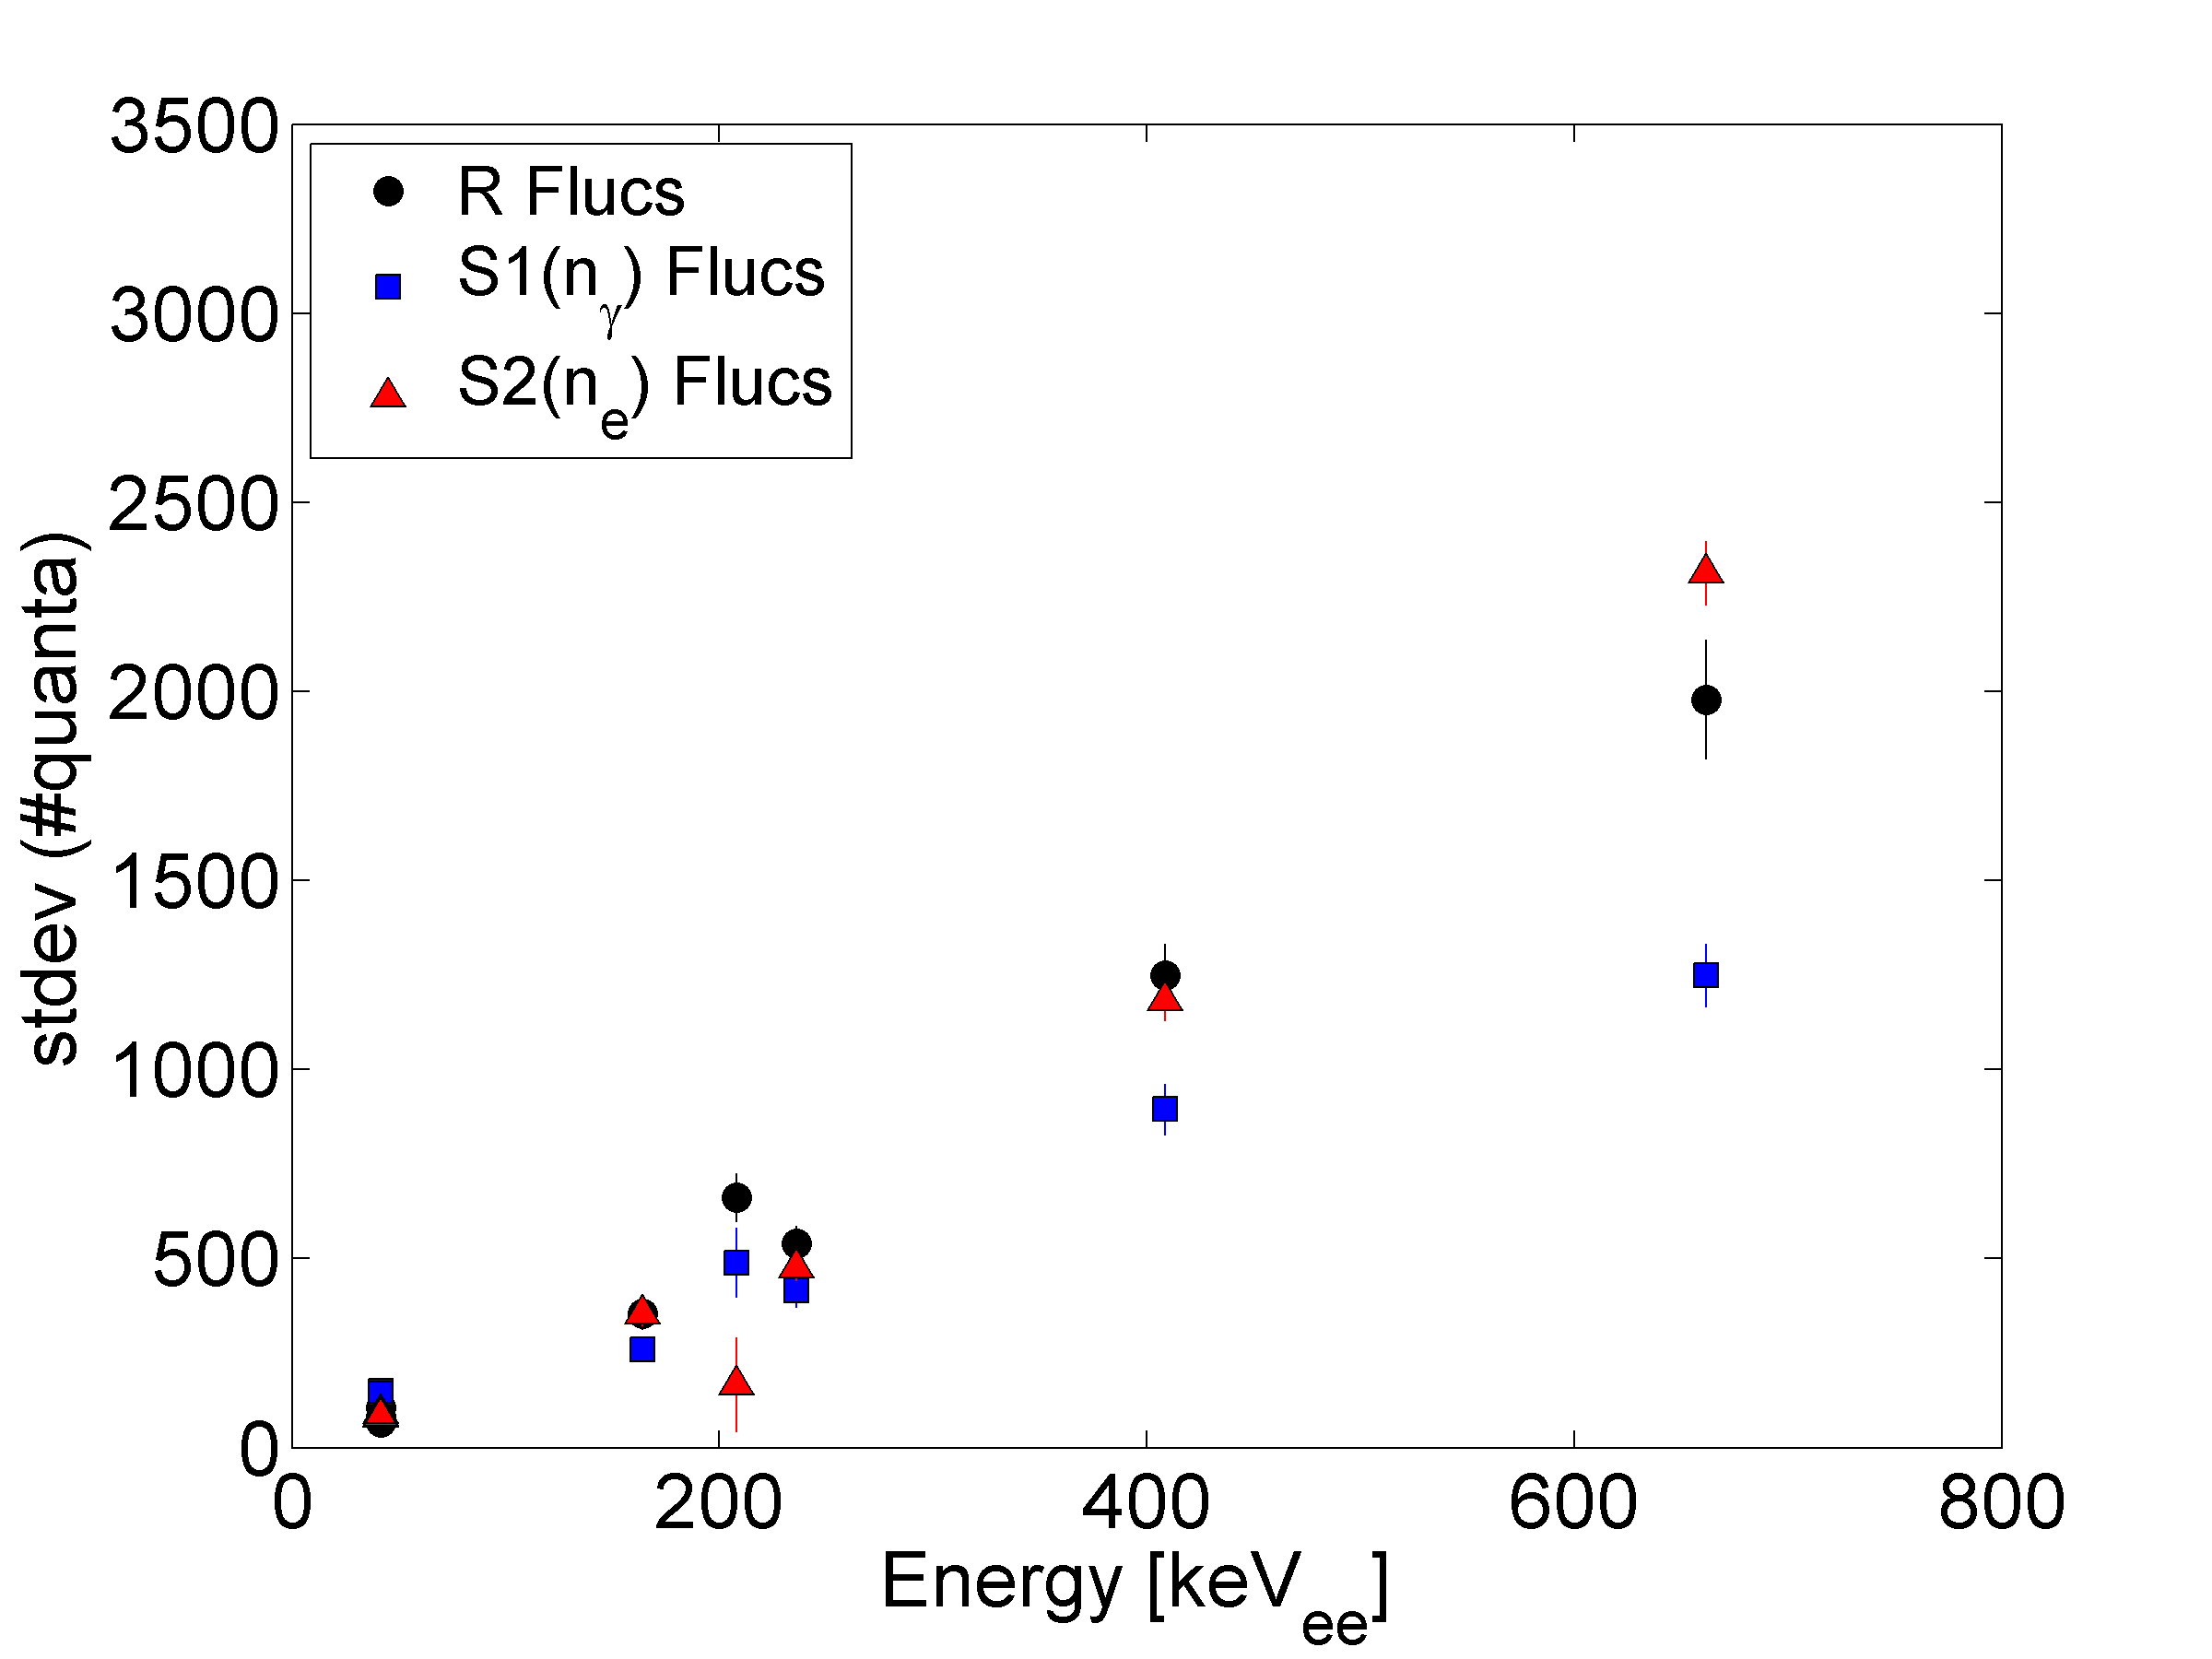
\includegraphics[scale=0.5]{EnergyFluctuations.png}
\caption{Measured values of $\sigma_{R}$, $\sigma_{n_{\gamma Det}}$, and $\sigma_{n_{e Det}}$ versus energy.}
\label{EnergyFluc}
\end{figure}

\begin{figure}[H]
\centering
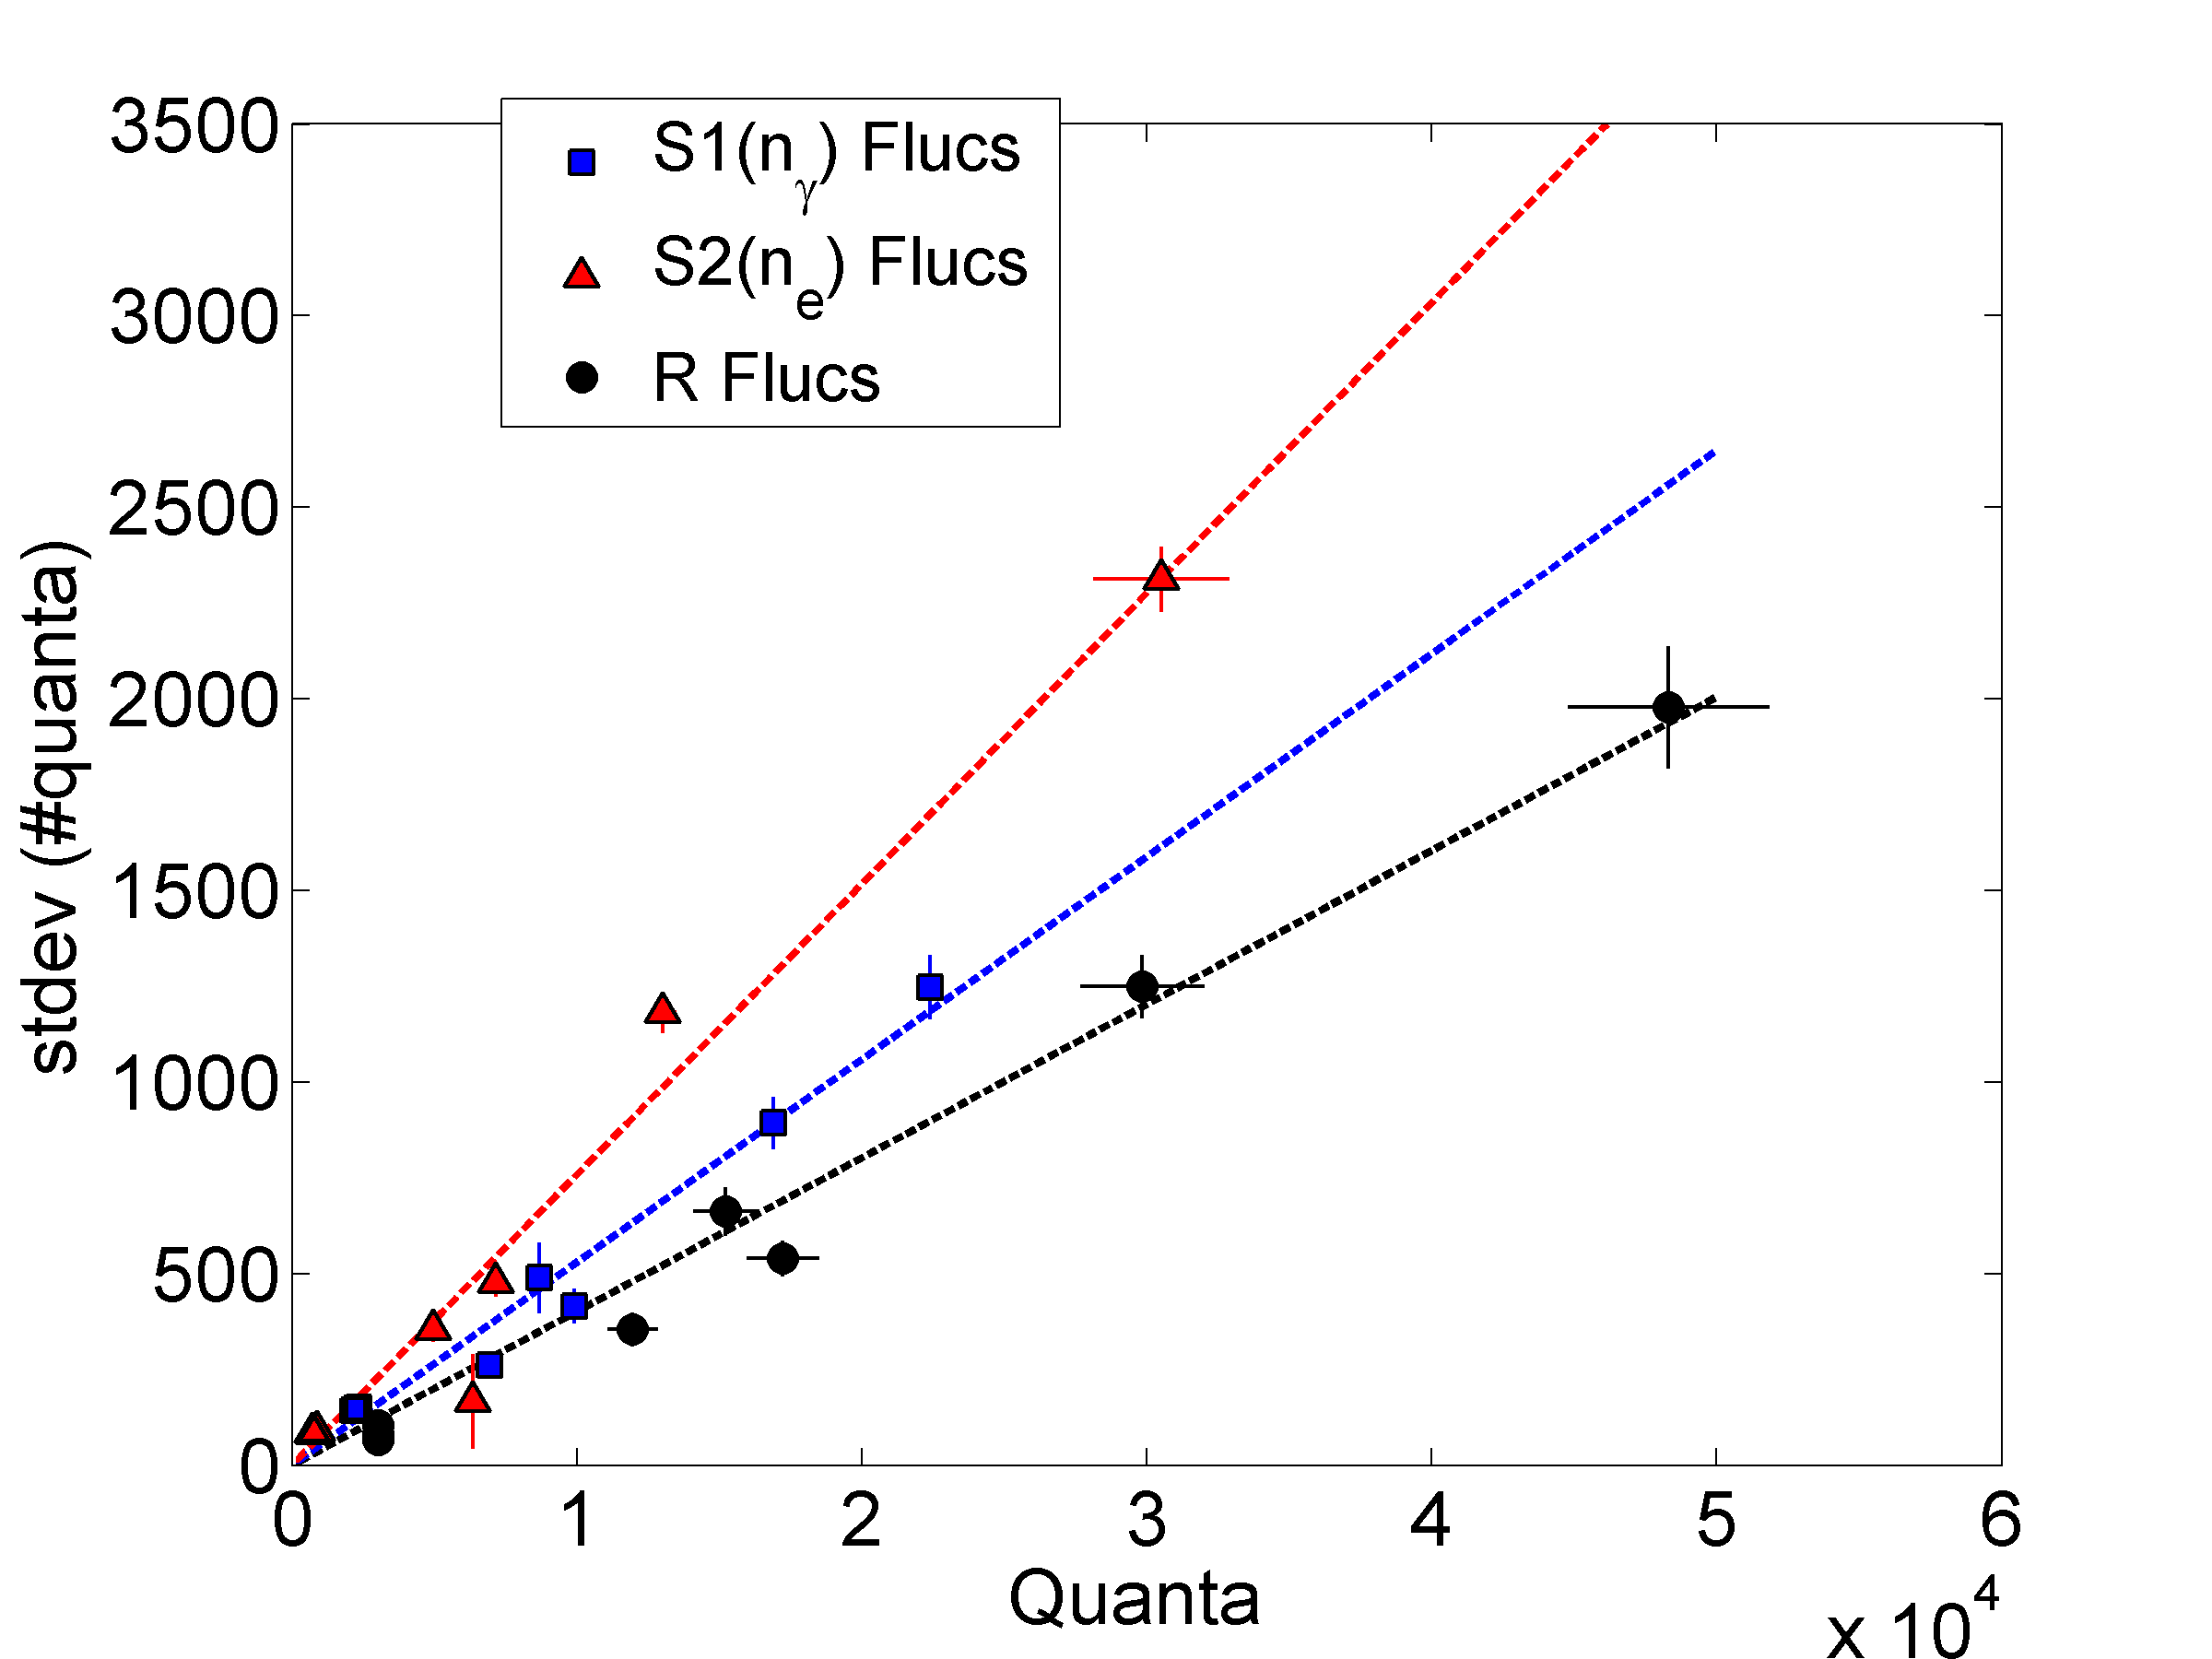
\includegraphics[scale=0.5]{QuantaFluctuations.png}
\caption{Measured values of $\sigma_{R}$, $\sigma_{n_{\gamma Det}}$, and $\sigma_{n_{e Det}}$ versus photons, electrons, and ions, respectively.}
\label{QuantaFluc}
\end{figure}

This study was repeated using the bottom PMT array only, while keeping both the cuts and fitting windows exactly the same.  The results are shown in Table~\ref{SigRBot}.  As expected the variance from recombination fluctuations appears independent of which PMTs are used in the analysis.  However, the slope of $\sigma_{n_{\gamma Det}}$ and $\sigma_{n_{e Det}}$ versus number of quanta is much more shallow when using the bottom PMT array only.  This could represent a systematic error, but it may also suggest that the top array of PMTs is contributing a significant amount of noise, or that the overall variance due to detector resolution is proportional to the number of PMTs which are used.  

\begin{center}
\begin{table}[H]
\begin{tabular}{ | c| p{40mm} | c | c | c | }
\hline
Source & Energy [keV] & $\sigma_{R}$ & $\sigma_{n_{\gamma Det}}$ & $\sigma_{n_{e Det}}$ \\ \hline
$^{83m}$Kr & 41.55 (50 V/cm) & 63.32 $\pm$ 1.2 & 152.6 $\pm$ 0.2 & 79.2 $\pm$ 0.4\\  \hline
$^{83m}$Kr & 41.55 (100 V/cm) & 82.16 $\pm$ 1.6 & 153.0 $\pm$ 0.3 & 84.5 $\pm$ 0.5\\  \hline
$^{83m}$Kr & 41.55 (170 V/cm) & 103.4 $\pm$ 1.1 & 149.7 $\pm$ 0.3 & 78.0 $\pm$ 0.5\\  \hline
$^{131}$Xe & 163.9 & 372.0 $\pm$ 27.8 & 249.7 $\pm$ 32 & 313.7 $\pm$ 33\\  \hline
$^{127}$Xe & 208.3 & 696.9 $\pm$ 61 & 400.5 $\pm$ 110 & 306.7 $\pm$ 90\\  \hline
$^{129}$Xe & 236.1 & 595.8 $\pm$ 34 & 348.0 $\pm$ 51 & 412.8 $\pm$ 42\\  \hline
$^{127}$Xe & 409 & 1328  $\pm$ 56 & 790.9 $\pm$ 77 & 874.5 $\pm$ 60\\  \hline
$^{214}$Bi & 609 & 1811 $\pm$ 312 & 2101 $\pm$ 100 & 3253 $\pm$ 180\\  \hline
$^{137}$Cs & 661.6 & 2235 $\pm$ 74.9 & 773.1 $\pm$ 136.5 & 1657 $\pm$ 94\\ 
\hline
\end{tabular}
\caption{Extracted fluctuations from Doke plot data in units of quanta when using the bottom array only.}
\label{SigRBot}
\end{table}
\end{center}


\subsubsection{Light Yield from Doke Plot Data}

The light yield in terms of $\frac{S1}{keV}$ and $\frac{photons}{keV}$ for each line source is easily obtainable from the Gaussian fits used in the Doke plot analysis and is included in~\ref{LY}.  In the case of $^{83m}$Kr two S1s (32.1 keV and 9.5 keV) are typically merged into one 41.55 keV S1 pulse by the data processing module.  The second of the two decays will occur with varying amounts of recombination depending on the amount of time between the first and second decay.  This recombination variation makes the combined 41.55 keV S1 pulse undesirable for measuring light yield.  Instead, we search for events where the two S1s occur far enough apart in time that data processing separates them into two S1 pulses.  A Gaussian fit is then used to determine the light yield from the 32.1 keV $^{83m}$Kr S1, resulting in 5.69 $\pm$ 0.03 $\frac{S1}{keV}$ and 46.3 $\pm$ 1.16 $\frac{photons}{keV}$. Note that the $^{127}$Xe 208.3 keV line in~\ref{LY} is still a result of two decays that are combined in our data processing, and this may affect the LY measurement for that point.

\begin{center}
\begin{table}[H]
\begin{tabular}{ | c | c | c | c |}
\hline
Source & Energy[keV] & $\frac{S1}{keV}$ & $\frac{photons}{keV}$ \\ \hline
$^{83m}$Kr & 32.1 (170 V/cm) & 5.69$\pm$0.03(5.62$\pm$0.36) & 46.3$\pm$1.16(45.7$\pm$3.13) \\  \hline
$^{131}$Xe & 163.9 & 5.08$\pm$0.05 & 41.3$\pm$1.1\\  \hline
$^{127}$Xe & 208.3(203+5.3) & 5.00$\pm$ 0.07 & 40.7$\pm$ 1.2\\  \hline
$^{129}$Xe & 236.1 & 5.04$\pm$ 0.04 & 41.0$\pm$ 1.1\\  \hline
$^{127}$Xe & 409 & 4.97$\pm$ 0.04 & 40.4$\pm$ 1.0\\  \hline
$^{214}$Bi & 609 & 4.21$\pm$ 0.03 & 34.2$\pm$ 0.9\\  \hline
$^{137}$Cs & 661.6 & 4.07$\pm$ 0.03 & 33.1$\pm$ 0.9\\ 
\hline
\end{tabular}
\caption{Light yield measurements from Doke plot data.}
\label{LY}
\end{table}
\end{center}

%Maybe plot LY v Energy Here

\subsection{Tritium $\chi^2$ Analysis of g$_1$ and g$_2$}

LUX's CH$_3$T calibration source produces a wide beta spectrum which continuously spans energies from the detector's threshold up to 18.6 keV.  We can take advantage of the wide energy spectrum to measure the g$_1$ and g$_2$ gain factors by varying g$_1$ and g$_2$ in a two dimensional $\chi^2$ fit until data matches the expected tritium beta spectrum.  References~\cite{TritiumSpec,TritiumSpec2,TritiumSpec3} derive an expression for the density of energy states accessible to the electron in a beta decay.  In terms of the kinetic energy of the electron, $T$, it is given by
\begin{equation} \label{TritiumBetaShape}
\frac{dN(T,Z)}{dT} = C(T^2 + 2Tm_e)^{1/2}(T+m_e)(Q-T)^2F(T,Z)
\end{equation}
where $Q_T=18.6 keV$ is the maximum kinetic energy of the electron, $m_e=511 keV$ is the mass of the electron, $C$ is a normalization constant, $Z=2$ is the nuclear charge for tritium, and 
\begin{equation}
F(T,Z) = 2\pi \frac{\alpha}{\left( \frac{\gamma^2 -1 }{\gamma^2}\right) ^{1/2}} 
\end{equation}
is the Coulomb correction due to nuclear charge with using $\alpha=1/137$ as the fine structure constant, and
\begin{equation}
\gamma = \frac{T+m_e}{m_e}
\end{equation}
as the energy to rest mass ratio.

Before using Equation~\ref{TritiumBetaShape} to produce the expected tritium beta spectrum in the LUX detector, we need to smear the distribution to model effects from the detector's resolution and recombination variation.  This is accomplished by drawing the true energy of events from the distribution described by~\ref{TritiumBetaShape} and feeding them into the NEST simulation package.  NEST produces simulated S1 and S2 signals for the corresponding energy deposition, which in turn provide a simulated tritium energy spectrum for the LUX detector using Equation~\ref{EnergyOne}.

Once we have a simulated model for the tritium energy spectrum in LUX we can minimize a two dimensional $\chi^2$ fit between the data and simulation to find the optimal values of g$_1$ and g$_2$.  The optimized CH$_3$T energy spectrum for the largest CH$_3$ calibration in LUX's Run03 data taking campaign is shown in Figure~\ref{TritiumSpectrum}.	The result of g1=0.115 $\pm$ 0.005 phd/photon, g2= 12.1 $\pm$ 0.9 phd/electron, and EE = 50.9\% $\pm$ 3.8\% is in close agreement with the Doke plot results from Section~\ref{DokePlot}.
